\section{Data}
\label{sec:data}
In the study, the main stock market indices were selected to represent the stock market indices of MINT and G7 countries. As can seen from Table~\ref{tab:variable}, FTSE MIB index for Italy, BIST 100 index for Turkiye, CAC 40 index for France, FTSE 100 index for UK, DAX PERFORMANCE index for Germany, S\&P 500 index for USA, S\&P/TSX index for Canada, IDX COMPOSITE index for Indonesia, IPC MEXICO index for Mexico, NIKKEI 225 index for Japan, and lastly NSE 30 index for Nigeria were chosen.  

To perform data analysis, we used daily closing prices for the indices accessed from https://finance.yahoo.com/ and https://www.investing.com. The data were collected from January 30, 2012 to August 14, 2024. The unavailability of old values of NSE 30 index was effective in the selection of this date range. After gathering data, the BIST 100 index was adjusted before the analysis because it reached 100,000 points on June 13, 2017, and two zeros were removed from the index as of July 27, 2020. For this reason, before July 27, 2020, we divided all values by 100 for BIST 100 index. 

When the descriptive statistics in Table~\ref{tab:descriptive} evaluated, even all indices ara non-normal, it is noteworthy that the BIST 100 and NSE 30 indices, which belong to MINT countries, are most positively skewed and leptokurtic.

All stock market indices values during that time were drawn in Figure~\ref{fig:alldata} for each country. According to Figure~\ref{fig:alldata}, although some dates are different, stock market movements seem generally similar because of the wide range of the y-axis. The decline in all of them, especially during the Covid period, is striking.

In addition to all data summaries, Spearman correlation analysis was also applied to indices to examine their relations between themselves. According to Figure~\ref{fig:cor2},  among MINT countries, Nigeria’s stock index was found to be least correlated with the other countries' indices, Mexico's index was second least correlated, and T\"{u}rkiye’s and Indonesia’s were most related. Nonetheless, because the dataset has time-dependent relationships, to use more appropriate method, dynamic time warping (DTW) was also used besides the Spearman correlation analysis. DTW is a robust approach to determine the distance which can be thought of as similarity measure between two time series, which may vary in time. The primary concept of DTW is to calculate the distance by comparing corresponding items in time series that are similar ~\citep{dynamic}. Unlike traditional distance measures, such as Euclidean distance, DTW can handle shifts and distortions in the time axis and calculates a cumulative distance by considering the minimum distance path through the cost matrix ~\citep{muller2007dynamic}. Lower DTW distances, generally close to 0 ones, indicate that the two time series are more similar. Thus, we can say according to Figure~\ref{fig:dist2}, except for the UK's and Indonesia's indices, most indices were very similar to the other countries' indices during the 12-year span.

\begin{table*}
    \caption{Variable explanations.}
      \label{tab:variable}
      \centering
    \scalebox{0.9}{
\begin{tabular}{@{}ll@{}}
\toprule
\textit{Variable} & \textit{Explanation} \\ \midrule
FTSE MIB   & Price performance of the 40 most-traded stock classes on the Borsa Italiana \\
BIST 100  & Price performance of the 100 largest companies on the Istanbul Stock Exchange \\
CAC 40    & Price performance the 40 most significant stocks on the Euronext Paris\\
FTSE 100   &Price performance of 100 most highly capitalised companies listed on the London Stock Exchange \\
DAX  PERFORMANCE   &Price performance of 30 biggest German companies that trade on the Frankfurt Exchange \\
S\&P 500    & Price performance of 500 of the largest companies listed on stock exchanges in the United States \\
S\&P/TSX    & Stock market index representing roughly 70\% of the total market capitalization on the Toronto Stock Exchange \\
IDX COMPOSITE  & Index of all stocks listed on the Indonesia Stock Exchange \\
IPC MEXICO  &Weighted measurement index of 35 stocks traded on the Borsa Mexico\\
NIKKEI 225   &Stock market index for the Tokyo Stock Exchange\\
NSE 30   &Price performance of 30 companies on the Nigerian Stock Exchange \\ \bottomrule
\end{tabular}
}
\end{table*}

\begin{table*}
    \caption{Descriptive statistics.}
    \label{tab:descriptive}
    \centering
    \scalebox{0.92}{
\begin{tabular}{@{}llllllllll@{}}
\toprule
\textit{Variable} & \textit{Source} & \textit{Size} & \textit{Mean} & \textit{Median} & \textit{Standard Deviation} & \textit{Minimum} & \textit{Maximum} & \textit{Skewness} & \textit{Kurtosis} \\ \midrule
FTSE MIB     & Yahoo Finance       & 4580       & 21732         & 21494           & 4422.896                    & 12358            & 35401            & 0.713             & 3.590             \\
BIST 100   & Yahoo Finance         & 4580       & 1969        & 977           & 2393.542                    & 541            & 11194          & 2.336             & 7.395             \\
CAC 40       & Yahoo Finance       & 4580       & 5308          & 5139            & 1216.689                    & 2929             & 8242             & 0.423             & 2.417             \\
FTSE 100     & Yahoo Finance       & 4580       & 6914          & 7004            & 644.245                     & 4994             & 8446             & -0.329            & 2.439             \\
DAX         & Yahoo Finance       & 4580       & 11990         & 12101           & 2865.310                     & 5976             & 18875            & 0.112             & 2.475             \\
S\&P 500     & Yahoo Finance       & 4580       & 2886          & 2680            & 1102.271                    & 1278             & 5644             & 0.526             & 2.149             \\
S\&P/TSX         & Yahoo Finance       & 4580       & 16280         & 15582           & 2957.038                    & 11310            & 23105            & 0.439             & 2.098             \\
IDX COMPOSITE        & Yahoo Finance       & 4580       & 5671          & 5779            & 961.285                     & 3697             & 7422             & -0.022            & 1.832             \\
IPC  MEXICO      & Yahoo Finance        & 4580       & 45960         & 45181           & 5118.520                     & 33338            & 58856            & 0.205             & 2.407             \\
NIKKEI 225    & Yahoo Finance      & 4580       & 21605         & 21103           & 7127.358                    & 8279             & 42344            & 0.376             & 2.909             \\
NSE 30      & Investing        & 4580       & 1635          & 1579            & 584.534                     & 872              & 3984             & 2.095             & 8.217             \\ \bottomrule
\end{tabular}
}
\end{table*}

\begin{figure*}
    \centering
    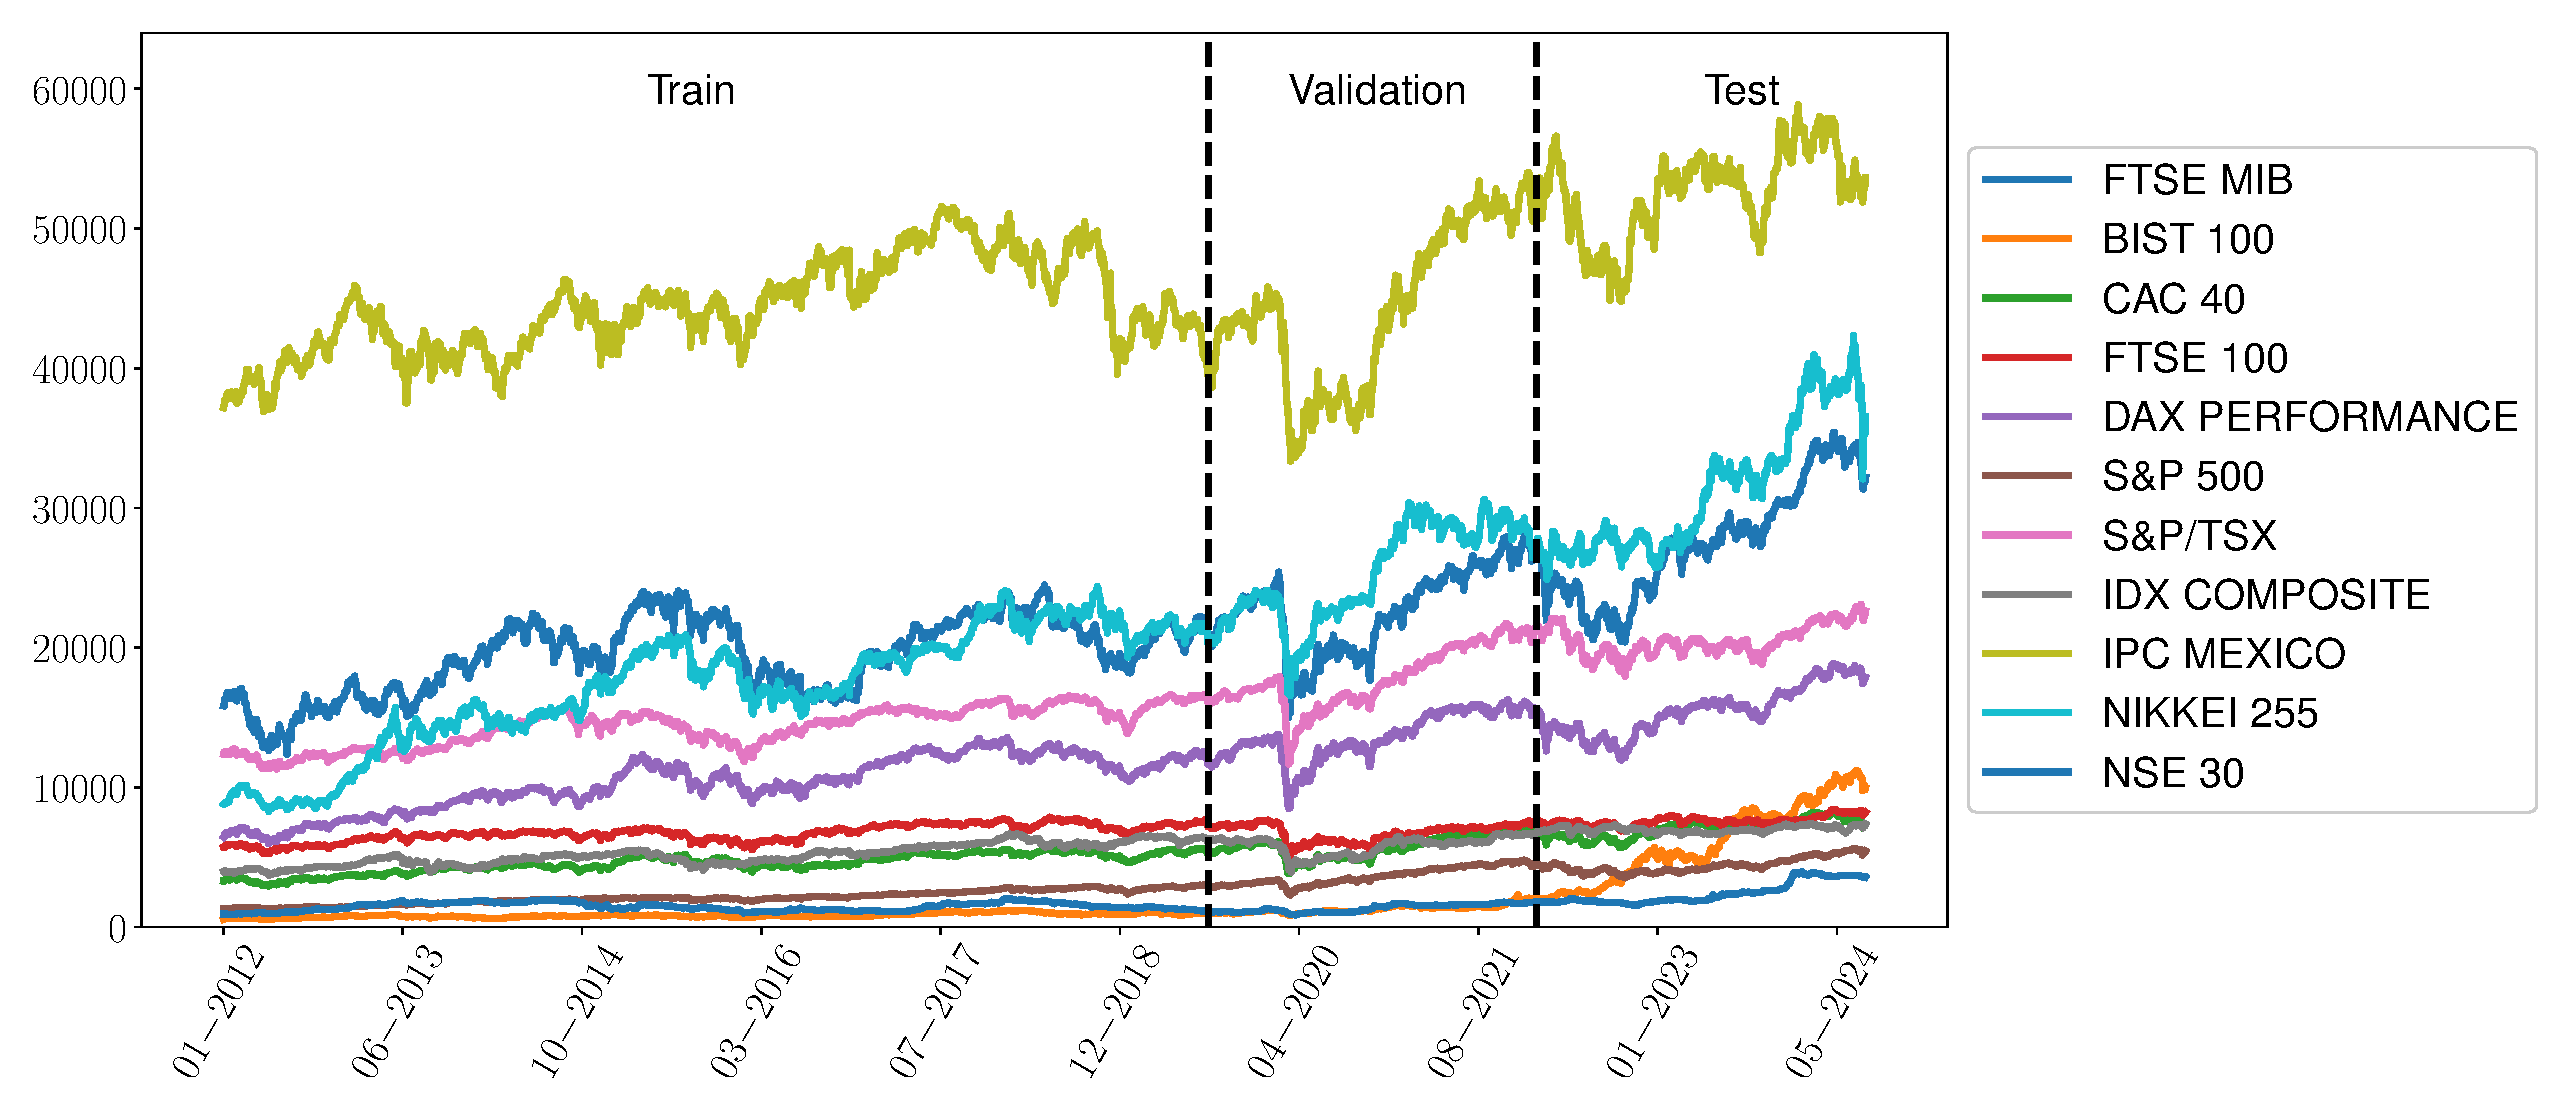
\includegraphics[width=1.0\textwidth]{./figures/alldata.eps}
    \caption{Daily closing price of the stock indices.}
    \label{fig:alldata}
\end{figure*}

\begin{figure}[tbh]
  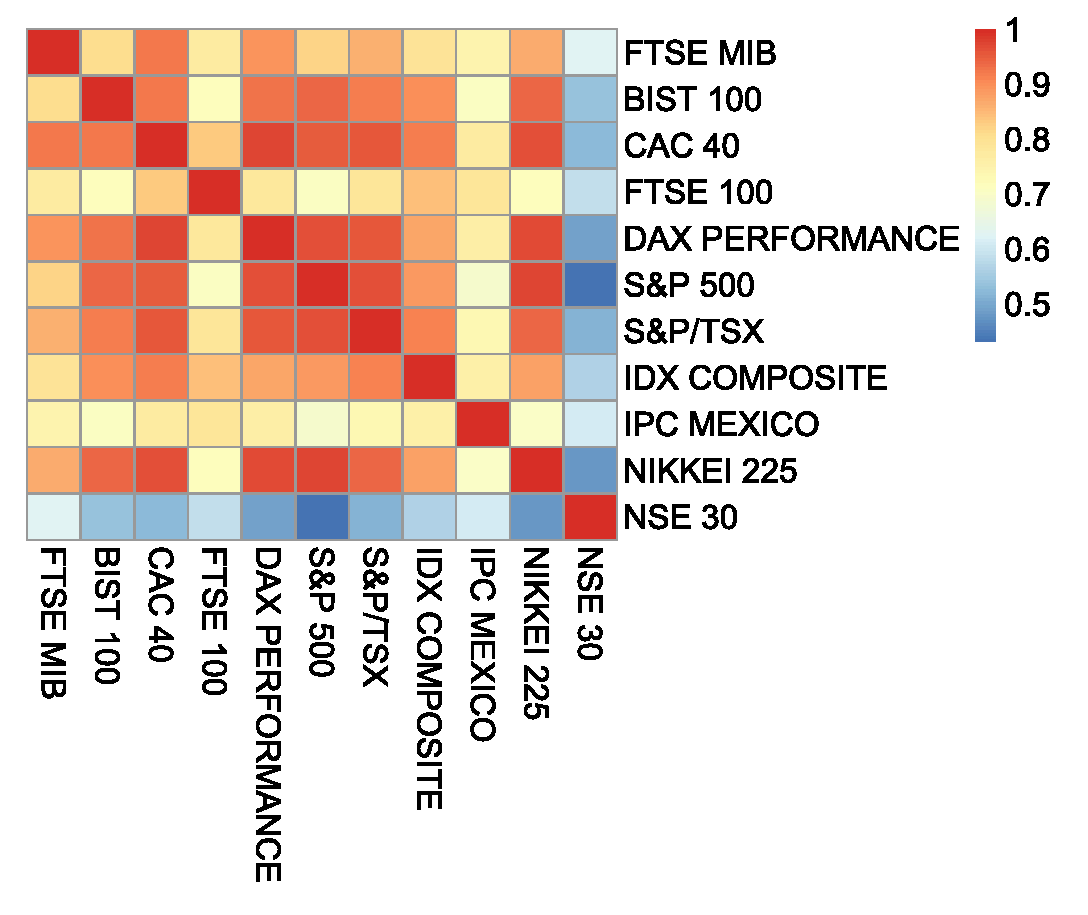
\includegraphics[width=0.47\textwidth]{./figures/cor2.eps}
  \caption{Correlation matrix.} 
  \label{fig:cor2}
\end{figure}

\begin{figure}[tbh]
  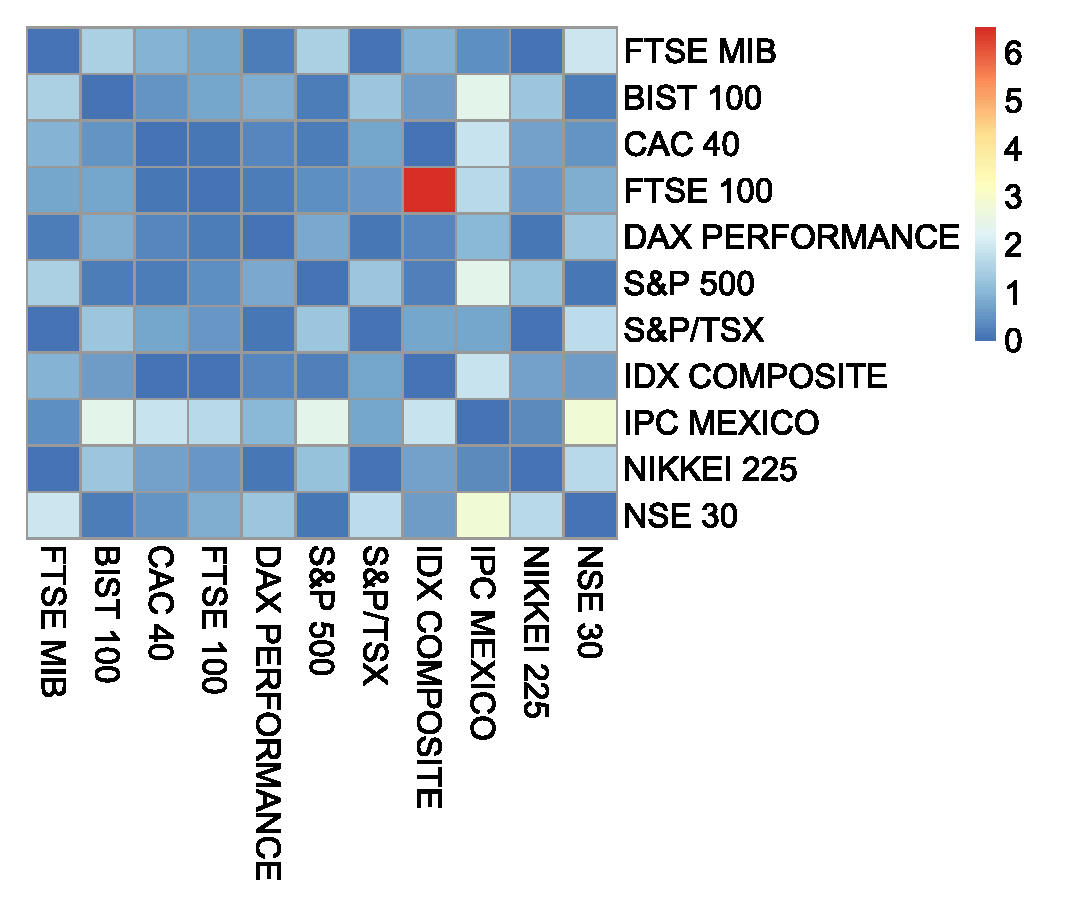
\includegraphics[width=0.47\textwidth]{./figures/dist2.eps}
  \caption{Distance matrix.} 
  \label{fig:dist2}
\end{figure}